\documentclass[../main/report.tex]{subfiles}
\begin{document}

\chapter{Testing}

Does it work?


\section{Component testing}
The system consists of a number of fairly isolated components.
It's valuable to test the components in isolation before they are connected.
Both implementation errors, and design flaws, can be uncovered before the components are introduced to the system.
The unit tests were implemented as VHDL test benches
Table \ref{tab:vhdl_unit_tests} describes the unit tests that was run.
\begin{table}[H]
	\centering
	\begin{tabularx}{\textwidth}{|c|X|c|}
	\hline
	\multicolumn{3}{|c|}{Unit tests.} \\
	\hline  Component under test & What is tested  	  & Status \\ 
	\hline  \multirow{3}{*}{Barrel selector} 		  & Barrel row is incremented each clock cycle.  & \multirow{3}{*}{ Passed } \\
	 										 		  & Barrow row wraps around to 0. & \\			
	 										 		  & PC write enabled high on row 0.& \\								
	\hline  \multirow{2}{*}{Constant memory} 	      & Constants can be written.  & \multirow{2}{*}{ Passed } \\
	 										 		  & Constants can be read. & \\												
	\hline \multirow{2}{*}{Inst decode/Control unit}  & Decodes instruction types correctly. & \multirow{2}{*}{ Passed } \\
		   											  & Sets control signal values correctly. &\\
	\hline \multirow{2}{*}{Instruction memory} 		  & Instructions can be written. & \multirow{2}{*}{ Passed } \\
													  & Instructions are read from the correct address  & \\ 
	\hline \multirow{2}{*}{Instruction memory} 		  & Instructions can be written. & \multirow{2}{*}{ Passed } \\
													  & Instructions are read from the correct address.  & \\ 
	\hline \multirow{3}{*}{Register file} 		  	  & Read/write to general purpose registers. & \multirow{3}{*}{ Passed } \\
													  & Dedicated registers behave correctly.  & \\ 
													  & Does the masking bit work.  & \\ 													  
	\hline  Register directory 		 				  & Multiplexes input/output signals to the correct register file. & Passed  \\
	
	\hline \multirow{3}{*}{Processor core} 		  	  & Arithmetic operations. & \multirow{3}{*}{ Passed } \\
													  & Can mask instructions.  & \\ 
													  
	\hline \multirow{3}{*}{ALU} 		  			  & Computes arithmetic operations. & \multirow{3}{*}{ Passed } \\
													  & Can do left/right shifts.  & \\ 
													  & Performs \emph{Set if les than} correctly. &	\\								  											  
	\hline
	\end{tabularx} 
	\caption{Unit tests for components in the Demolicious system.}
	\label{tab:vhdl_unit_tests}
\end{table}
\section{VHDL system integration tests}

Before deploying to an actual FPGA, it is important to ensure correct behavior in system-level testbenches.
This testing is valuable, as if one can verify correct behavior in simulation, one has fewer potential errors when debugging the FPGA itself.

System tests for each of the major datapaths through the design have been created and run successfully.
The result of each test is verified by comparing all pixels in the framebuffer after the kernel has been run, to precomputed values in Isim.


\subsection{Memory stores and kernel parameterization}

To verify that stores to memory, as well as constant memory, actually works, the kernel presented in listing \ref{lst:param-color-kernel} is used as a system test.
It has been relisted in listing \ref{lst:test-param-kernel} for convenience.
If successful, this allows for parameterizing kernel behaviour with values loaded at runtime, reducing the need for recompilation.

\begin{assembly}[caption={Kernel to test constant memory and parameterization}, label=lst:test-param-kernel]
ldc $data, 0
mv $address_lo, $id_lo
mv $address_hi, $id_hi
sw
thread_finished
\end{assembly}

Expected behavior of test:
\begin{enumerate}
  \item
    The color green should successfully be loaded from constant memory.
  \item
    It should be stored to memory.
  \item
    The screen should be filled with the color green.
\end{enumerate}

\subsubsection*{simulation results}

\begin{figure}[H]
  \centering
  \begin{subfigure}[b]{\textwidth}
    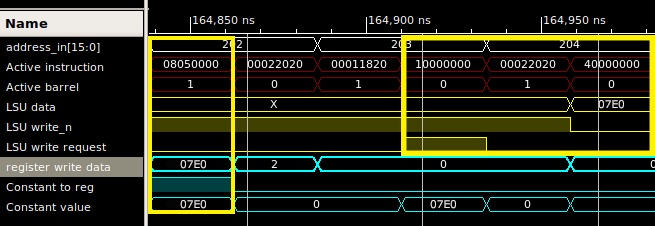
\includegraphics[width=\textwidth]{../testing/assets/Constant_load_&_store.png}
    \caption{Isim simulation showing constant load and store word}
    \label{fig:isim-kernel-parameterization}
  \end{subfigure}
  \begin{subfigure}[b]{0.3\textwidth}
    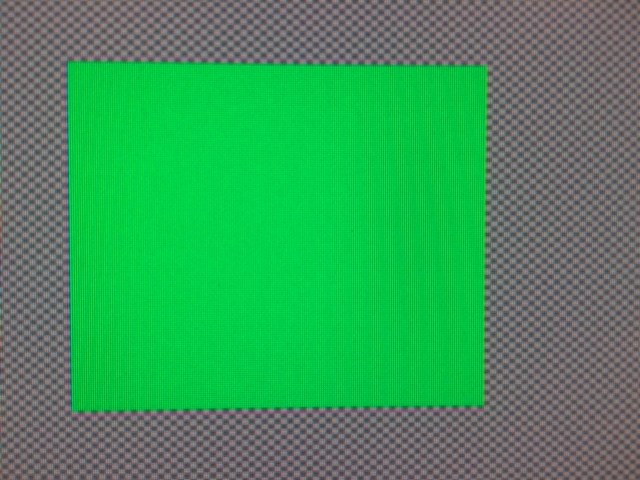
\includegraphics[width=\textwidth]{../testing/assets/green_screen.jpg}
    \caption{LX16 run}
    \label{fig:LX16-kernel-parameterization}
  \end{subfigure}
  \caption{Results from simulation and LX16 of fillscreen kernel}
\end{figure}

In the left yellow square of figure \ref{fig:isim-kernel-parameterization}, one can see the load constant instruction being executed (0x08050000) in barrel line 1.
The Constant to reg signal is asserted, and the constant value 0x07E0 is passed into the register write data signal.

In the right yellow square, the store word instruction (0x100000000) executes in barrel line 0.
The LSU accepts the write request same cycle (LSU write request goes high), and two cycles later the request packet reaches the LSU data line.
The LSU asserts LSU write\_n, (the signal is active low), and external RAM handles the store request.

The testbench passes, and values have now been successfully written to memory.
It also runs on actual hardware, the result shown in figure \ref{fig:LX16-kernel-parameterization}.

\subsection{Masked instruction execution}

Masked instructions are used to allow for some degree of conditional execution in the lack of proper branching and jumps.
This requires that the architecture actually respects the mask bit when set.
The masked execution kernel presented earlier in listing \ref{lst:lst:masked-execution} is used for this test.
It has been relisted in listing \ref{lst:test-masked-execution} for convenience.

\begin{assembly}[caption=Conditional execution using predicated instructions, label=lst:test-masked-execution]
ldc $10, 0 ; Load color one
ldc $11, 1 ; Load color two
srl $mask, $id_lo, 6 ; Shift to the right converts ID to y pos
mv $data, $10
? mv $data, $11 ; Will only be executed every other row
mv $address_lo, $id_lo
mv $address_hi, $id_hi
sw
thread_finished
\end{assembly}

Expected behavior of test:
\begin{enumerate}
  \item
    Each row should be colored according to the last bit of their y position.
\end{enumerate}

\subsubsection*{simulation results}

\begin{figure}[H]
  \centering
  \begin{subfigure}[b]{\textwidth}
    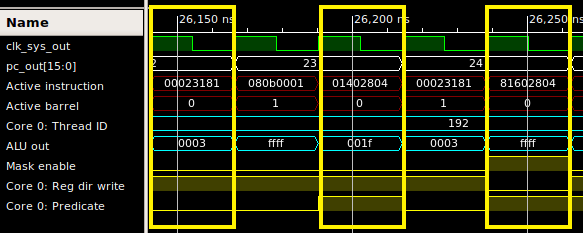
\includegraphics[width=\textwidth]{../testing/assets/masking-yes.png}
    \caption{Isim simulation showing successful masking.}
    \label{fig:isim-masked-execution}
  \end{subfigure}
  \begin{subfigure}[b]{0.3\textwidth}
    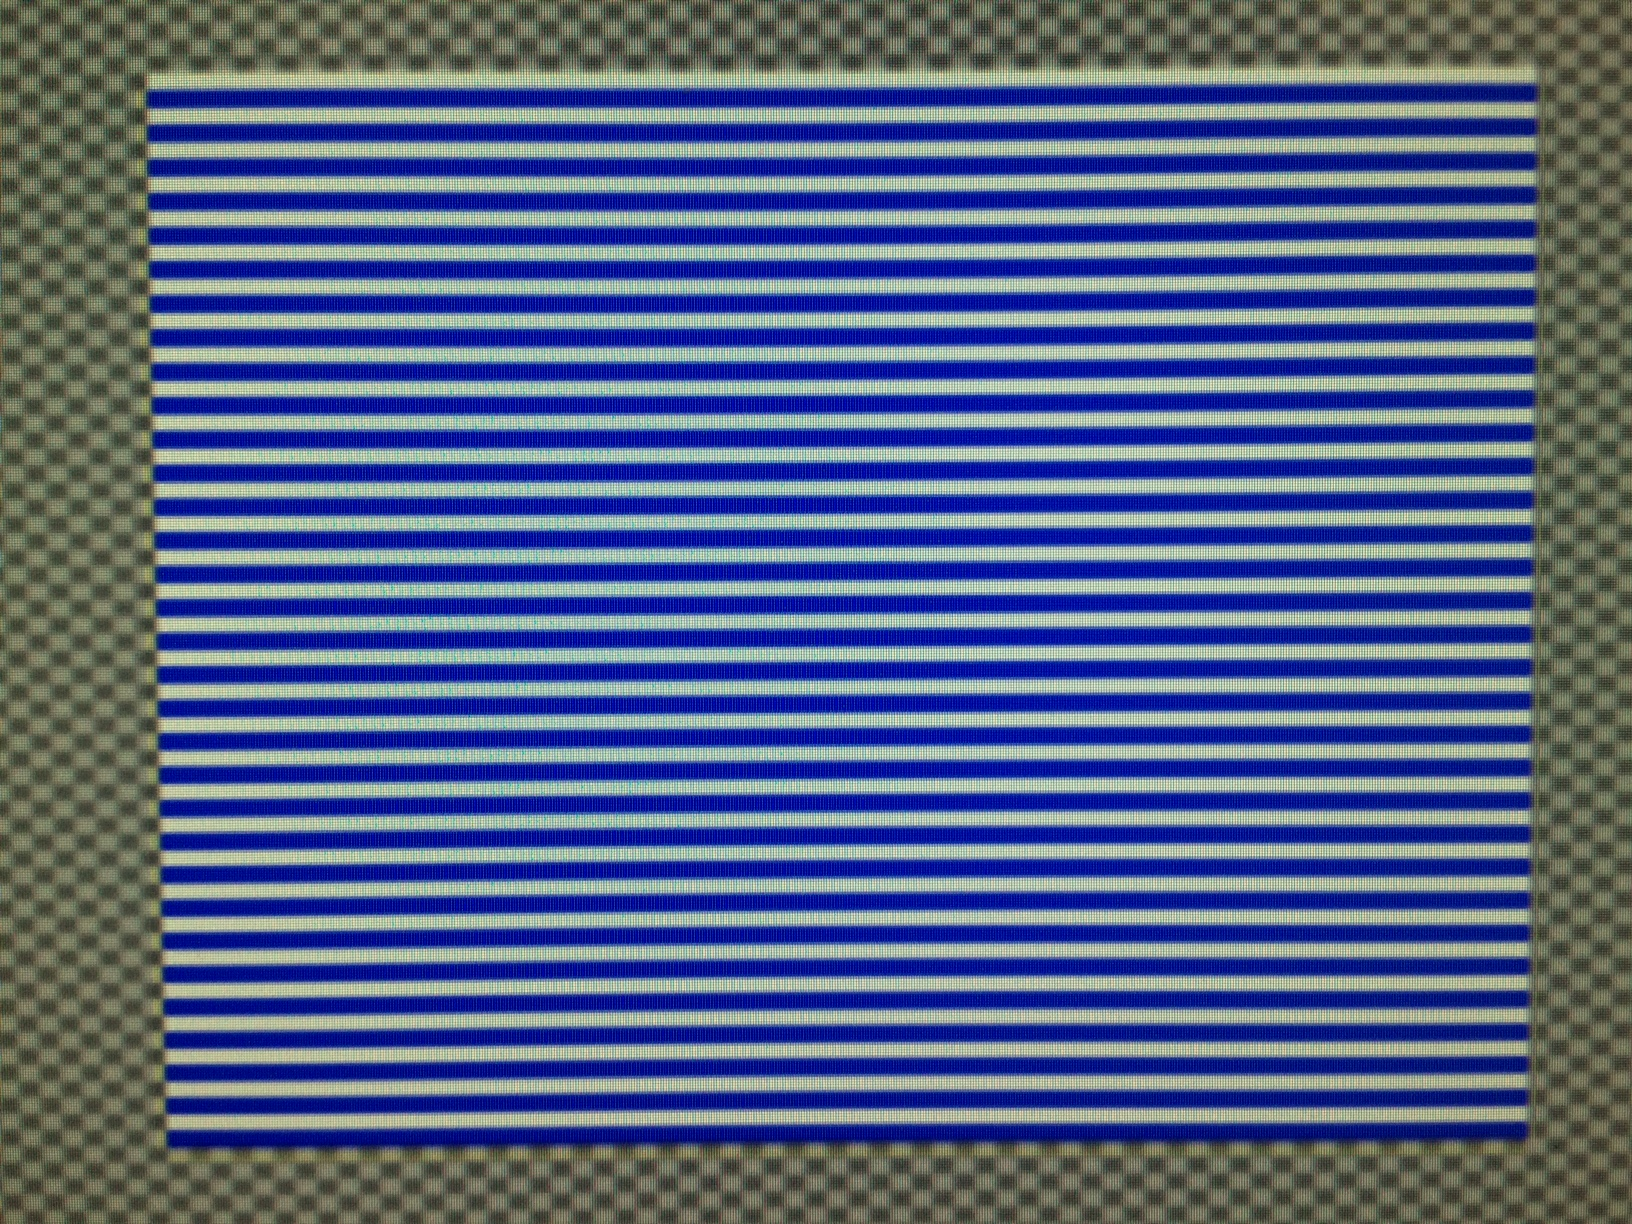
\includegraphics[width=\textwidth]{../testing/assets/lines.jpg}
    \caption{LX16 run}
    \label{fig:LX16-masked-execution}
  \end{subfigure}
  \caption{Results from simulation and LX16 of masked execution}
\end{figure}

In the left yellow square of figure \ref{fig:isim-masked-execution}, we can see the \verb/srl/ instruction being executed (0x00023181). As this thread has thread id 192, the result out is 3.
The low bit is stored into the mask register, enabling masking for this thread.

In the middle yellow square, barrel 0 is once again active, and we can see that the predicate bit of core 0 has been asserted.
As this instruction isn't masked, the predicate bit is ignored and the value of 001f is stored into the data register.

In the right yellow square, the conditional data move is executed (0x81602804).
As the mask enable signal goes high, the register write enable signal is pulled low due to the predicate bit, resulting in the data not being written to registers.

The testbench passes, and predicated instructions are not executed when masking is enabled.
As can be seen in figure \ref{fig:LX16-masked-execution}, the kernel runs on actual hardware, and every second line is colored differently.

\subsection{Loads from primary memory}

\subsection{Kernel square}


\subfile{../testing/io_testing.tex}


\section{PCB tests}

After receiving the finished PCB and the components, we performed the following tests before reaching a final (hardware-wise)functional computer.   

\subsection{Solder, signal and power test}
The purpose of these tests was to solder components and checking that their connections held, as well as checking that power correctly propagated through the board.  
\subfile{../testing/Solder_test.tex}

\subsection{Oscillator and clock test}
These tests consisted of using an oscilloscope in order to probe the outputs of the FPGA's oscillator and the high frequency and low frequency crystals.
\subfile{../testing/oscillation_test.tex}

%\subsection{JTAG test}
%In these tests we attempted to connect to respectively, the FPGA and the MCU by way of the appropriate headers, thereby verifying that they had been properly soldered in place and were functional.
%\subfile{../testing/JTAG_test.tex}

\end{document}
